\chapter{Modulació $\Sigma \Delta$}
\section{Disseny i evaluació de la topologia del modulador $\Sigma\Delta$}
\par En aquest treball, s'ha optat per implementar una etapa de modulació $\Sigma\Delta$ com estratègia per fer més efectiu el rebuig del soroll que incorporen les mostres d'àudio per diversos efectes, e.g. el procés de quantització. S'estudien els efectes d'implementar un modulador $\Sigma\Delta$ de segon ordre amb realimentació negativa,i com a referència per a la posterior comparació, es prenen els càlculs presentats a l'apartat 4.7 per un modulador $\Sigma\Delta$ de primer ordre. 
\par Un dels principals motius per fer l'estudi d'un modulador de segon ordre, és la implementació aparentment trivial a la FPGA degut a la manca de coeficients a diferència d'altres topologies (veure apartat 4.7). No obstant, la presència de dos llaços de realimentació i dos integradors en el modulador $\Sigma\Delta$ de segon ordre, comporta una possible deriva de l'estabilitat del sistema si no es prenen les consideracions adequades. A la figura \ref{fig_SigmaDelta} es pot visualitzar l'estructura que es pretén implementar, on els blocs H(z) representen els integradors i els valors $a_1$,$a_2$ els coeficients de pre-acondicionament.
\begin{figure}[H]
    \centering
    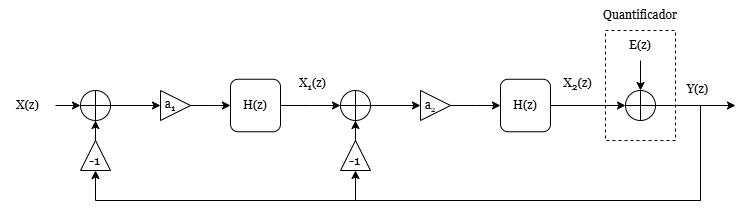
\includegraphics[width=0.7\linewidth]{Images/SigmaDelta.drawio.png}
    \caption{Diagrama de blocs d'un modulador $\Sigma\Delta$ de segon ordre.}
    \label{fig_SigmaDelta}
\end{figure}
\par De la figura \ref{fig_SigmaDelta}, cal destacar com el bloc Quantificador es pot modelar com la addició d'un senyal d'error E(z) assumint que el procés és lineal. Aquesta última aproximació de l'error de quantificació permet modelitzar el tractament del soroll i caracteritzar la resposta en freqüència. 
\par En el disseny d'aquest modulador $\Sigma \Delta$, el quantificador de la sortida és de 2 nivells amb una rebuig del soroll de quantificació esperat de 70 dB. Amb l'equació \ref{eq_SQNR}, es troba que per complir les especificacions s'ha de produir un sobremostreig de OSR = 32. Per tant, de \cite{UndrstndSDM} es defineix que la freqüència de mostreig a l'entrada del modulador amb $f_B$ = 20 kHz, ha de ser de:
\begin{equation}
    f_{s_{min}} = 2\ OSR\ f_B = 1,28\ MHz
\end{equation}
\par La seqüència de sortida està representada per Y(z) i la sortida de cada integrador ve donada per la seva variable d'estat, $X_1$(z) i $X_2$(z) per al primer i el segon integrador, respectivament. El sistema d'equacions es pot escriure de la següent forma:
\begin{equation}\label{eq_sistemaSDM}
    \left\lbrace\begin{array}{c}  X_1(z) = a_1 H(z) (X(z)-Y(z)) \\ X_2(z) = a_2 H(z) (X_1(z)-Y(z)) \\
    Y(z) = X_2(z) + E(z)\end{array}\right.
\end{equation}
Resolguent el sistema \ref{eq_sistemaSDM}, es troba que la funció de transferència del Senyal (STF) i del Soroll (NTF) s'expressen de la següent forma:
\begin{equation}\label{eq_STF}
    STF(z) = \frac{a_1 a_2 H^{2}(z)}{a_1 a_2 H^{2}(z) + a_2 H(z) + 1}
\end{equation}
\begin{equation}\label{eq_NTF}
    NTF(z) = \frac{1}{a_1 a_2 H^{2}(z) + a_2 H(z) + 1}
\end{equation}
\par Per poder trobar el valor dels coeficients de pre-acondicionament, cal estudiar l'estabilitat del sistema en temps continu. Per tant, s'analitza el sistema amb la variable de Laplace (s) i es considera la funció de transferència del bloc integrador com:
\begin{equation}\label{eq_intLaplace}
  H(s) = \frac{1}{T_s s}  
\end{equation} 
\par Les equacions \ref{eq_STF} i \ref{eq_NTF} es poden transformar a la variable de Laplace simplement substituint el bloc integrador per l'equació \ref{eq_intLaplace}. Per evaluar l'estabilitat del sistema, es troba que el denominador de la funció de transferència s'expressa de la següent forma:
\begin{equation}\label{eq_dentransf}
    D(s) = s^2 + \frac{a_2}{T_s} s + \frac{a_1 a_2}{T_s}
\end{equation}
\par Aplicant el criteri de Routh-Hurwitz, el sistema és estable per $a_1$, $a_2$ $>$ 0. Com a \cite{ADC16b}, s'assigna als coeficients de pre-acondicionament $a_1$=$a_2$=0,5 degut a que en operacions binàries el producte per $\frac{1}{2}$ equival a desplaçar el vector de bits 1 bit a l'esquerra.
\par Tornant de nou al temps discret, la funció de transferència dels blocs integradors en la variable z ve donada per:
\begin{equation}\label{eq_IntZ}
    H(z) = \frac{z^{-1}}{1 - z^{-1} }
\end{equation}
\par Amb els nous valors de $a_1$ i $a_2$, i la funció de transferència \ref{eq_IntZ}, les funcions de transferència \ref{eq_STF} i \ref{eq_NTF} resulten en: 
\begin{equation}\label{eq_STFsimpl}
    STF(z) = \frac{z^{-2}}{3z^{-2}-6z^{-1}+4}
\end{equation}
\begin{equation}\label{eq_NTFsimpl}
    NTF(z) = \frac{(1-z^{-1})^2}{3z^{-2}-6z^{-1}+4}
\end{equation}
\par Es pot observar a \ref{eq_STFsimpl} com el senyal d'entrada està retardada 2 mostres ($z^{-2}$), mentres l'error de quantificació està modelat pel terme (1-$z^{-1}$)$^2$ \cite{ADC16b}. Les expressions \ref{eq_STFsimpl} i \ref{eq_NTFsimpl} representen un filtre passa-baixos de les mostres samplejades i un filtre passa-alts per l'error de quantificació, respectivament. Aquest comportament caracteritza els moduladors $\Sigma \Delta$, ja que permet filtrar el senyal d'interès en la banda de pas, desplaçant l'error de quantificació cap a freqüències més altes. Això contribueix a una millora significativa de la relació senyal-soroll (SNR) del senyal portador d'àudio, fet que es tradueix en una qualitat sonora superior. 
\par Per analitzar l'estabilitat del sistema implementat i poder valorar la resposta en freqüència, es resolen les arrels del denominador de \ref{eq_STFsimpl} i \ref{eq_NTFsimpl}:
\begin{equation}\label{eq_polesSTF}
    0 = 4z^{2}-6z+3 \longrightarrow z_p = \frac{3}{4} \pm \frac{\sqrt{3}}{4}i
\end{equation}
\begin{equation}\label{eq_module_poleszSTF}
    \left|z_p\right| = \frac{\sqrt{3}}{2} = 0,866
\end{equation}
\begin{equation}\label{eq_angle_poleszSTF}
    \left|\theta_p\right| = 0,523\ rad
\end{equation}
\begin{figure}[H]
    \centering
    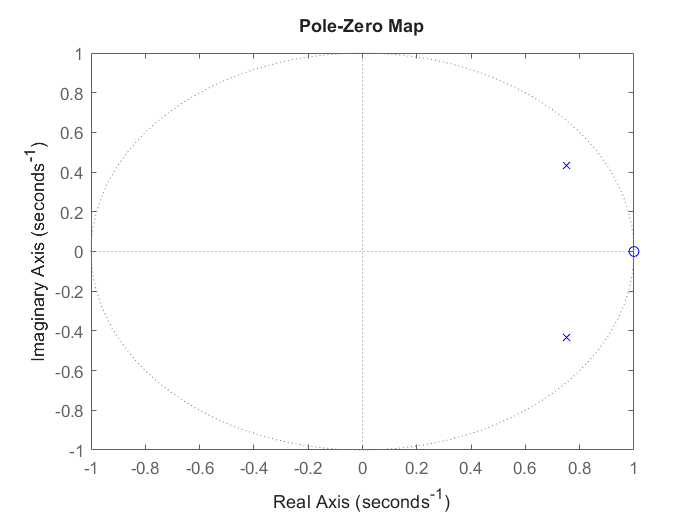
\includegraphics[width=0.5\linewidth]{Images/zeropoleMapMOD2.png}
    \caption{Cercle unitari en el pla polar de STF(z) i NTF(z). STF(z) i NTF(z) comparteixen pols.}
    \label{figzeropoleMap}
\end{figure}
\par Amb \ref{eq_module_poleszSTF} es pot verificar que els pols estan ubicats dins del cercle unitari, i per tant, es dedueix que el sistema es estable aparentment. Addicionalment, es possible trobar la freqüència que s'amplifica en la banda de pas tant de la funció de transferència del senyal d'entrada (STF) com en la del modelat del soroll (NTF), a partir de l'angle dels pols respecte l'eix real del pla polar (\ref{eq_angle_poleszSTF}). Només cal fer la transformació de freqüència en rad/mostra a Hz aplicant una simple regla de tres.
\begin{equation}\label{eq_cornerfreq}
    f_{peak} = \frac{\theta_{p}}{2\pi}\ f_{sample} = \frac{0,523}{2\pi}1,41\times 10^6 = 117,46\ kHz
\end{equation}
\begin{equation}\label{eq_magn_wnSTF}
    \left| STF(\theta_p)\right| = 6\ dB
\end{equation}
\begin{equation}\label{eq_magn_wnNTF}
    \left| NTF(\theta_p)\right| = 6,5\ dB
\end{equation}
\par Això ens permetrà dimensionar el sistema de forma més precisa per valorar posteriorment com es comporta el sistema en conjunt.
\par Per poder trobar la freqüència de tall del bloc es resol l'equació \ref{eq_STFsimpl} igualant-la a 0,707, que equival al decaïment de 3 dB en la banda de pas de la funció de transferència. S'aplica el mateix procediment a l'equació \ref{eq_NTFsimpl} per trobar a partir de quina freqüència deixa d'atenuar l'error de quantificació. 
\begin{equation}\label{eq_fcorteSTF}
    \left| STF(z)\right| = 0,707 \longrightarrow f_{c,STF} = 183,6\ kHz
\end{equation}
\begin{equation}\label{eq_fcorteNTF}
    \left| NTF(z)\right| = 0,707 \longrightarrow f_{c,NTF} = 77,95\ kHz
\end{equation}
\par Finalment, es procedeix a dimensionar el bloc $\Sigma \Delta$ de segon ordre dissenyat i s'exposen les característiques de rendiment a la taula \ref{taula_SigmaDelta}. 

\begin{table}[H]
    \centering
    \begin{tabular}{ | c | c | }
    \hline
    \centering
    SNQR     &  70.1 dB\\ \hline
    \centering
    DR    &    112,28 dB \\ \hline
    \centering
    OSR    &    32 \\ \hline
    \centering
    $fs_{in}$   &    1,41 MHz \\ \hline
    \centering
    $f_{tall, STF}$    &   183,6 kHz\\ \hline
    \centering
    $f_{tall, NTF}$    &   77,95 kHz\\ \hline
    \centering
    $f_{peak, STF}$    &   117,46 kHz\\ \hline
    \centering
    $f_{peak, NTF}$    &   117,46 kHz\\ \hline
    \end{tabular}
    \caption{Taula de les mètriques de rendiment calculades pel modulador $\Sigma \Delta$ dissenyat.}
    \label{taula_SigmaDelta}
\end{table}
\begin{figure}[H]
    \centering
    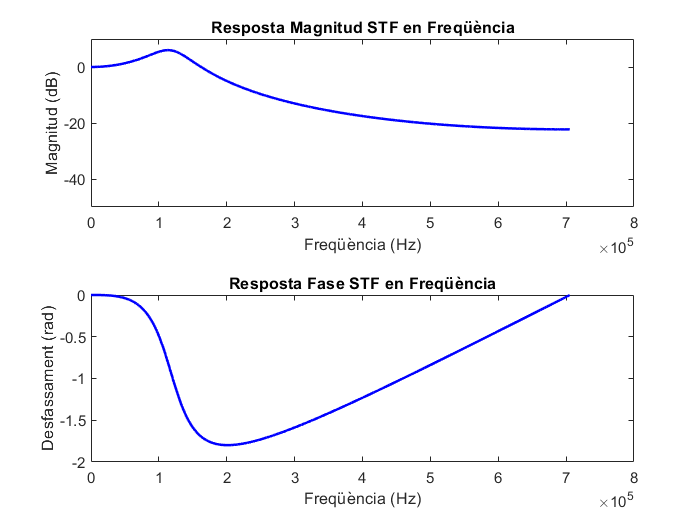
\includegraphics[width=0.5\linewidth]{Images/bodeSTFMOD2.png}
    \caption{Diagrama de Bode de la funció de transferència del Senyal (STF(z)).}
    \label{figbodeSTF}
\end{figure}
\begin{figure}[H]
    \centering
    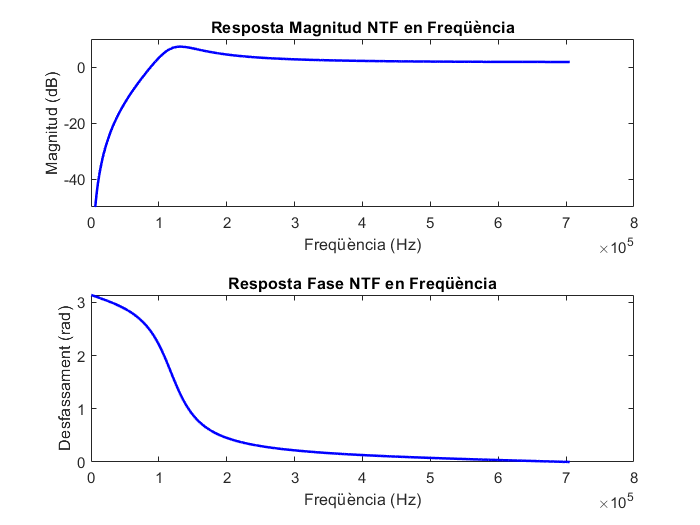
\includegraphics[width=0.5\linewidth]{Images/bodeNTFMOD2.png}
    \caption{Diagrama de Bode de la funció de transferència del Soroll (NTF(z)).}
    \label{figbodeNTF}
\end{figure}

\section{Implementació en codi VHDL}
\par Per a la implementació del modulador s'ha optat per descriure l'entitat en codi VHDL de forma intuïtiva per facilitar la feina de debugging en el procés de validació. 
\par L'estructura del bloc $\Sigma \Delta$ s'ha dissenyat dins de la mateixa sentència \textit{process}, amb només el senyal del rellotge de la FPGA a la llista de sensibilitat. D'aquesta forma, tots els subprocessos que es duen a terme en el modulador s'executen síncrons al rellotge intern de la FPGA. Seguint el diagrama de blocs de la figura \ref{fig_SigmaDelta}, el codi en VHDL s'ha agrupat en subblocs disposats d'esquerra a dreta. Aquesta organització permet tenir una visió més intuïtiva i coherent del que s'està implementant. El codi, tot i que és de creació pròpia, està inspirat en \cite{codiGit}.
\begin{figure}[H]
    \centering
    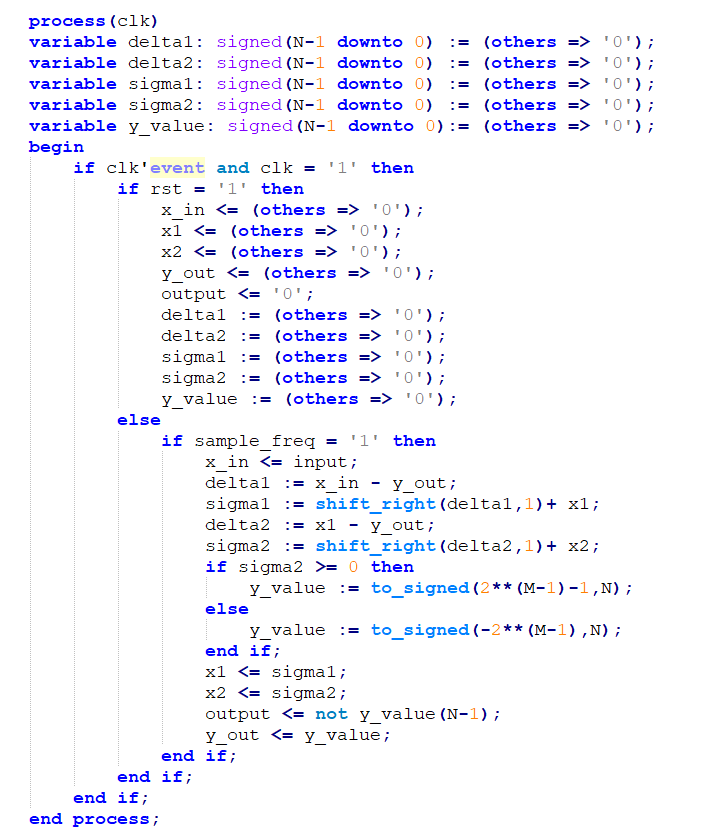
\includegraphics[width=0.5\linewidth]{Images/process_SDM.png}
    \caption{Sentència del \textit{process} on s'executen les operacions del modulador $\Sigma \Delta$.}
    \label{fig_processSDM}
\end{figure}
\begin{figure}[H]
    \centering
    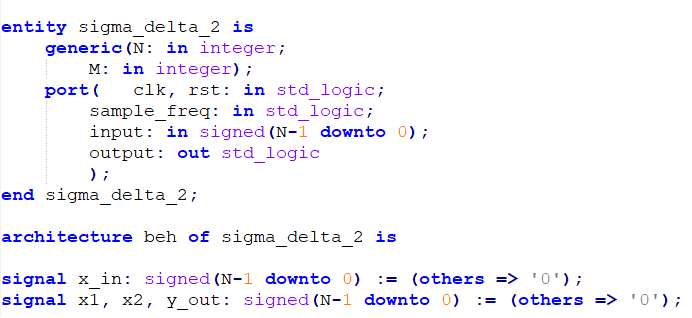
\includegraphics[width=0.5\linewidth]{Images/signals_SDM.png}
    \caption{Declaració de senyals de l'entitat sigma\textunderscore delta\textunderscore2}
    \label{fig_signalsSDM}
\end{figure}
\par Com es pot apreciar a la figura \ref{fig_SigmaDelta}, la sortida dels blocs $\Delta$ s'assigna a una variable \textit{deltaN} i la sortida dels blocs integradors o $\Sigma$, s'assignen a un senyal definida sota la nomenclatura de la variable d'estat visible a la figura \ref{fig_SigmaDelta}. En l'entorn VHDL, les variables dins d'un \textit{process} s'actualitzen en el mateix instant de canviar el seu contingut; no és el cas dels senyals, doncs en VHDL s'actualitzen un cop finalitzat el bloc \textit{process}. Per aquest motiu, els senyals que representen les variables d'estat s'actualitzen un cicle de mostreig més tard, tal i com està definit en l'equació \ref{eq_IntZ}. Per fer una abstracció del que s'està implementant, a la figura \ref{fig_integradordelay} es pot veure l'estructura del bloc integrador.
\begin{figure}[H]
    \centering
    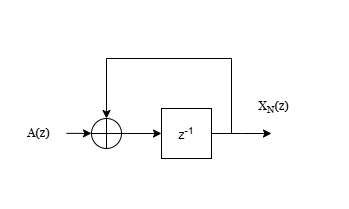
\includegraphics[width=0.5\linewidth]{Images/DelayIntegrator.png}
    \caption{Diagrama de blocs del bloc integrador del modulador $\Sigma \Delta$}
    \label{fig_integradordelay}
\end{figure}
\par El bloc quantificador està implementat de manera que pugui ser configurable el valor dels nivells i no hi hagi desbordament aritmètic en els blocs integradors. Modificant el valor genèric M, és possible definir inicialment el format en coma fixa dels valors a l'entrada. I finalment, la sortida del bloc $\Sigma \Delta$ prové del signe del valor en els llaços de realimentació. És a dir, si el valor al llaç és positiu a la sortida hi haurà un 1 lògic i si el valor al llaç de realimentació és negatiu, a la sortida PDM hi haurà un 0 lògic.

\subsubsection{Validació en testbench}
\par En l'última etapa de la validació del modulador, es dissenya un banc de proves per a l'entitat en VHDL. Per poder comprovar que efectivament el bloc funciona correctament, es genera un senyal sinusoidal de 24 bits amb un fons d'escala de 16 bits i es simulen el senyal de rellotge i el senyal corresponent a la freqüència de mostreig. 
\begin{figure}[H]
    \centering
    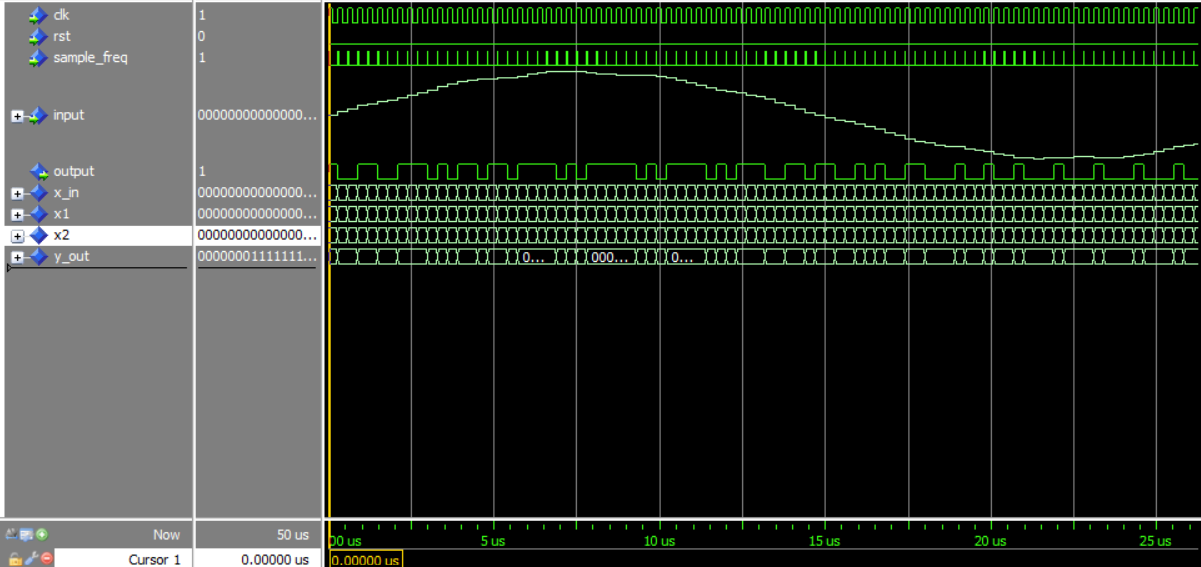
\includegraphics[width=0.7\linewidth]{Images/TestbenchSigmaDelta.png}
    \caption{Diagrama de temps del banc de proves per la validació de l'entitat sigma\textunderscore delta\textunderscore2. En gran es pot apreciar l'ona sinusoidal aplicada a l'entrada i abaix la sortida en format PDM del modulador.}
    \label{figtestbench_SigmaDelta}
\end{figure}
\begin{figure}[H]
    \centering
    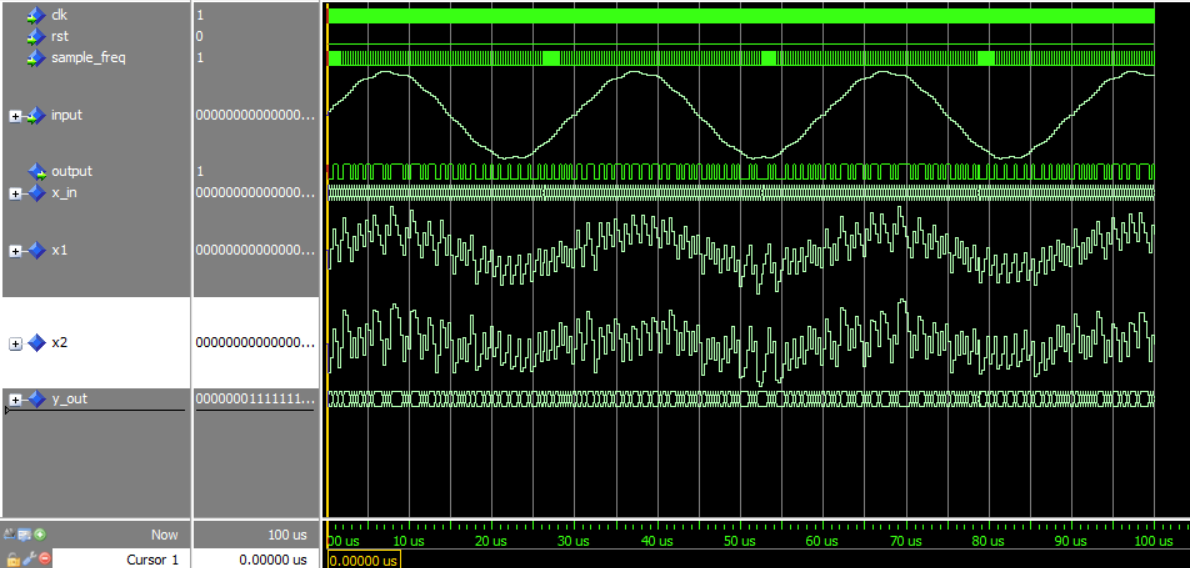
\includegraphics[width=0.7\linewidth]{Images/TestbenchSigmaDelta_integrator.png}
    \caption{Diagrama de temps del banc de proves per la validació de l'entitat sigma\textunderscore delta\textunderscore2. De nou, en gran es pot apreciar l'ona sinusoidal aplicada a l'entrada i més avall, les senyals x1 i x2 el valor de les variables d'estat.}
    \label{figtestbench_SigmaDelta2}
\end{figure}

\par Tal com es mostra a les figures \ref{figtestbench_SigmaDelta} i \ref{figtestbench_SigmaDelta2}, el bloc $\Sigma \Delta$ funciona segons el comportament esperat. A la sortida, es pot observar que l'amplada dels polsos varia en funció del senyal sinusoidal.

\section{Implementació a la FPGA}
\par Finalment, s'importa l'entitat dissenyada al programa Vivado per generar el bloc IP que posteriorment s'afegirà al projecte general. A la taula \ref{taularecursosSigma}, es pot visualitzar els recursos emprats de la FPGA per a la implementació del modulador. Destaquen les 228 LUTs i la manca de blocs DSP la qual cosa ens indica que el programa ha sintetitzat el blocs sumadors amb LUTs i registres. Pràctica que no resulta gaire eficient però degut a les dimensions del treball no suposa un impediment per a la implementació en conjunt. 

\begin{table}[H]
    \centering
    \begin{tabular}{ | c | c | c | c | c | c |}
    \hline
    \centering
    \textbf{ID}     &  \textbf{LUTs} & \textbf{Registres}  & \textbf{Slices} & \textbf{Muxes}  & \textbf{DSPs} \\ [2ex] \hline
    \centering
    sigma\textunderscore delta \textunderscore 2    &  228 & 67  & 32 & 0  & 0 \\ \hline
    \end{tabular}
    \caption{Utilització de recursos de la FPGA pel bloc IP dissenyat.}
    \label{taularecursosSigma}
\end{table}